\chapter{Cryo-EM and cryo-ET}

In this chapter, I describe the role of cryo-EM and cryo-ET in the field of structural biology, explain their fundamentals, and discuss advantages and limitations.

Structural biologists employ several techinques to understand the structure and function of biomolecular systems, typically proteins, nucleic acids and their ligands.
Arguably, the three giants in the field are X-ray crystallography, Nuclear Magnetic Resonance (NMR) and cryo-electron microscopy (cryo-EM), with several other techniques playing complementary, more specialized or niche roles (such as mass spectroscopy, neutron scattering or small-angle scattering).
Each technique has pros and cons, making it suited to different samples and applications.

In X-Ray crystallography --- in many ways the predecessor to cryo-EM as all-purpose structural biology technique --- crystals are grown from the sample of interest; the crystals are then illuminated by an X-ray beam, and the diffraction pattern thus created can be detected and used to reconstruct the three-dimensional (3D) structure of the sample.
Thanks to the short wavelength of X-rays --- as opposed to visible light --- it is possible to localize the positions of atoms with sub-angstrom precision CITE.
X-ray crystallography has played a major role in the development of structural biology, and is still the primary source of protein structures on the Protein Data Bank~\cite{bermanProteinDataBank2000,bermanAnnouncingWorldwideProtein2003}.
However, the need for crystallization poses a few limits.
The crystallization procedure is often hard to devise and reproduce, extending the time and resources needed for sample preparation.
Moreover, the resulting crystal "forces" the sample into a crystalline lattice, often with biologically irrelevant chemical states, restricting the conformational freedom of the molecule and limiting the biological significance of the obtained structures CITE.

\section[Cryo-EM and SPA]{Cryo-electron microscopy and single particle analysis}

Cryo-EM improves on these aspects, by using vitrification to capture the sample at a near-native state, and by forgoing crystallization and the analysis of diffraction patterns in favor of free single molecules and the use of the central slice theorem to combine many projections into a single 3D structure (known as single particle analysis or SPA).

(TODO: these base-concepts paragraphs here feel a bit out of place, I'm struggling to find where they should be and in what order...)

In simple terms, the electron microscope works by shooting a coherent electron beam at the sample, and using a camera to detect the scattered electrons and form an image.
Thanks to the small wavelength of electrons, cryo-EM can reach much higher resolution than light microscopy; however, it presents unique challenges and limitations that its more familiar light-based counterpart does not.

In the last decade, the development of direct electron detectors made it possible to reach atomic resolutions, jump-starting to the so-called resolution revolution and the rise of cryo-EM as one of the primary methods for high resolution structure determination~\cite{faruqiCCDDetectorsHighresolution2000}.

Differently from light-microscopy, which relies on amplitude contrast for image formation, the electron microscope uses phase contrast, which is caused by elastic scattering events affecting the electrons traversing the sample CITE.
Some electrons, however, are inelastically scattered; these electrons are no longer coherent, and therefore add to the noise of the image.
Increasing the electron dose can help improve the signal-to-noise ratio (SNR), but comes at the cost of radiation damage, which denatures the sample and rapidly destroy high-resolution information.
For these reasons, a significant limitation --- and thus optimization target --- of cryo-EM is the low SNR.

The cryo-EM workflow is well established, and usually consists of the same principal components: sample preparation and vitrification, data collection, preprocessing (cleaning, motion and CTF correction), particle picking and classification, three-dimensional (3D) reconstruction, and model building.
This section describes such typical workflow, expanding on the theoretical bases surrounding each step.

\subsection{Sample preparation}
Cryo-EM samples for SPA are usually prepared in vitro by expressing ad purifying the protein or complex of interest to create a minimal system.
Sample concentration and purity are important variables to control, as they will affect vitrification and data processing complexity.
The sample solution is then deposited on a cryo-em grid and vitrified via plunge freezing or other methods (\autoref{fig:plunge_freezing})(TODO: elaborate or just leave to citation?) CITE.
Vitrification allows to fixate the sample at near-native, hydrated conditions while avoiding the formation of crystalline ice, which would damage the sample CITE.
When vitrifying, the thickness of the ice is crucial: a thinner layer will results in fewer inelastically scattered electrons during data collection and better SNR.
However, too-thin ice can crack and increase issues with preferential orientation or particle distribution.

TODO: more about screening or is this enough?

\begin{figure}[ht]
    \centering
    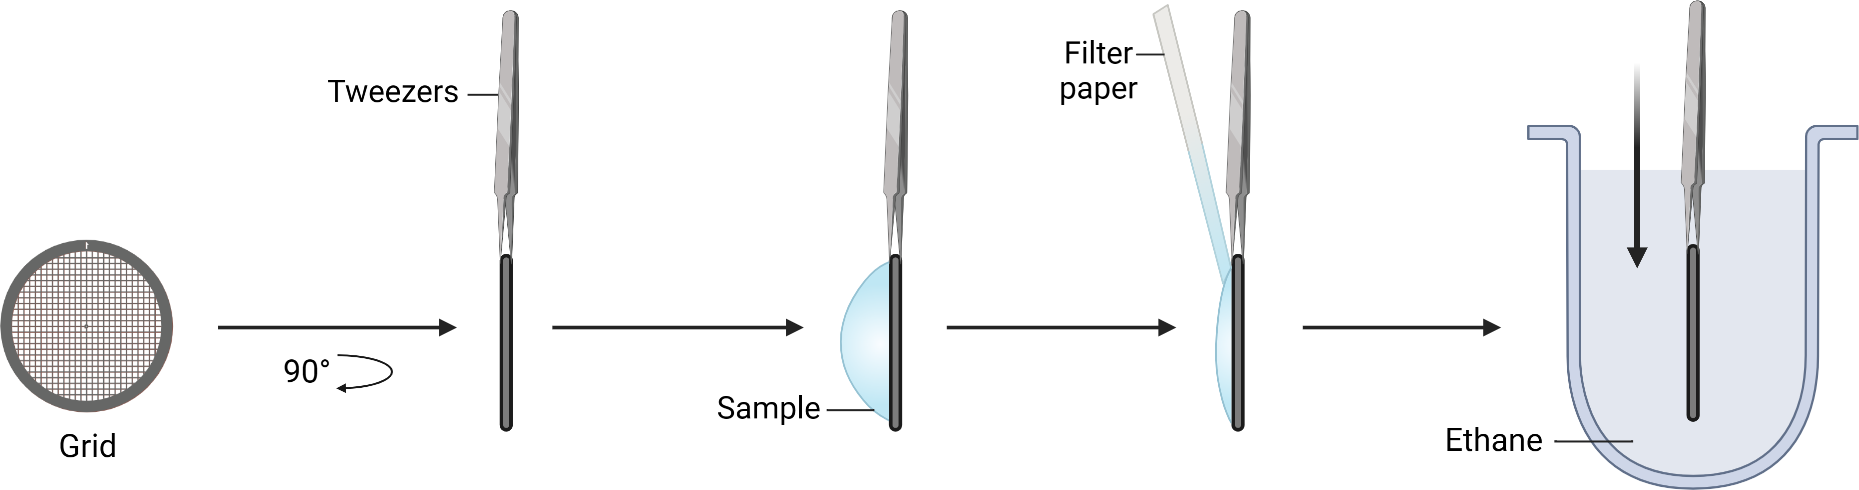
\includegraphics[width=\textwidth]{introduction/plunge_freezing.png}
    \caption[Vitrification via plunge freezing]{TODO: also, why ethane?. Figure adapted from \citet{chungNobelPrizeChemistry2017}.}
    \label{fig:plunge_freezing}
\end{figure}

\subsection{Data collection}
The vitrified sample is loaded into the electron microscope (under cryogenic conditions and vacuum, in order to maintain the sample vitrified and uncontaminated), and suitable positions on the grid are chosen for imaging, prioritizing for: presence of the target protein or complex, fewer contaminations, and lower ice thickness.
In modern workflows and software, this step and the subsequent data collection are increasingly automated, allowing for higher throughput (up to several thousand images per day) and lower human intervention CITE.

During collection, the sample stage and electron beam are moved to each position to collect micrographs.
At each position, a short movie is recorded, consisting of a few low-dose, short-exposure frames: this allows to reduce the blur caused by intra-frame motion (induced by external factors among which the electron beam itself); the frames will later be aligned and averaged to produce a single higher-contrast image.
Direct detectors are therefore crucial not only for their raw improvement in achievable resolution, but also for their high speed, contributing to the reduction of yet another source of noise.

(TODO: I'd like to add something like "There are many steps and challenges in the setup of a data collection; as this thesis does not focus on the experimental side, this part will be treated only superficially" or similar... not sure if/where)

An important concept to be mindful of when setting up a data collection is defocus; in order to better understand how defocus affects later processing steps, we first need to understand image formation in the electron microscope, and the importance of estimating and correcting the Contrast Transfer Function (CTF).

\subsubsection{Image formation and CTF}

In electron microscopy, image contrast derives almost entirely from phase contrast (CITE and/or expand about phase vs amplitude contrast).
The electron beam generated by the microscope is initially coherent, that is the phases of all the electrons in the beam are correlated.
When electrons traverse the sample, they have a chance to undergo elastic scattering; this results in a shift in the electron's phase, leading to interference with the unscattered wave at the image plane (\autoref{fig:image_formation}).
It's this interference that create phase contrast and ultimately the image.

Some electrons are also inelastically scattered: these electrons lose energy and coherence, and are therefore adding to the noise of the image because the lenses no longer focus them to the right place.
To mitigate this effect, inelastically scattered electrons are filtered out using an energy filter, which removes electrons with energy that differs significantly from the unscattered ones (\autoref{fig:image_formation}).

Inelastic scattering is also the source of radiation damage: the energy lost by these electrons is transferred to the sample, denaturing and deforming it and thus affecting SRN.

\begin{figure}[ht]
    \centering
    \includegraphics[width=.5\textwidth]{example-image.png}
    \caption[Image formation in cryo-EM]{TODO: add image of electron beam and image formation}
    \label{fig:image_formation}
\end{figure}

The CTF is a function that describes how signal is transmitted through the sample and onto the image, as a function of spatial frequency.
Specifically, the CTF is a parametrized sinusoidal function that approximates the power spectrum (PS) of the image, that is: the absolute value of the fourier transform of the image.

The CTF is usually described as composed of two main elements: the oscillating one responsible for phase contrast, and the envelope function, a dampening effect which attenuates the signal at higher resolutions and depends on many factors, such as spatial frequency, lens aberrations, and limitations of the electron gun.
Where the CTF reaches a value of \num{0}, no signal is transferred; a value of \num{1}, on the other hand, is a perfect signal transfer.

The oscillating component of the CTF is an intrinsic aspect of how phase contrast is achieved via constructive and destructive interference of scattered and non-scattered electrons.
Its exact shape depends on several factors, first among which the defocus: a different defocus value will shift the zeros of the CTF, nullifying different spatial frequencies (\autoref{fig:ctf_defocus}).

\begin{figure}[ht]
    \centering
    \begin{subfigure}{.6\textwidth}
        \centering
        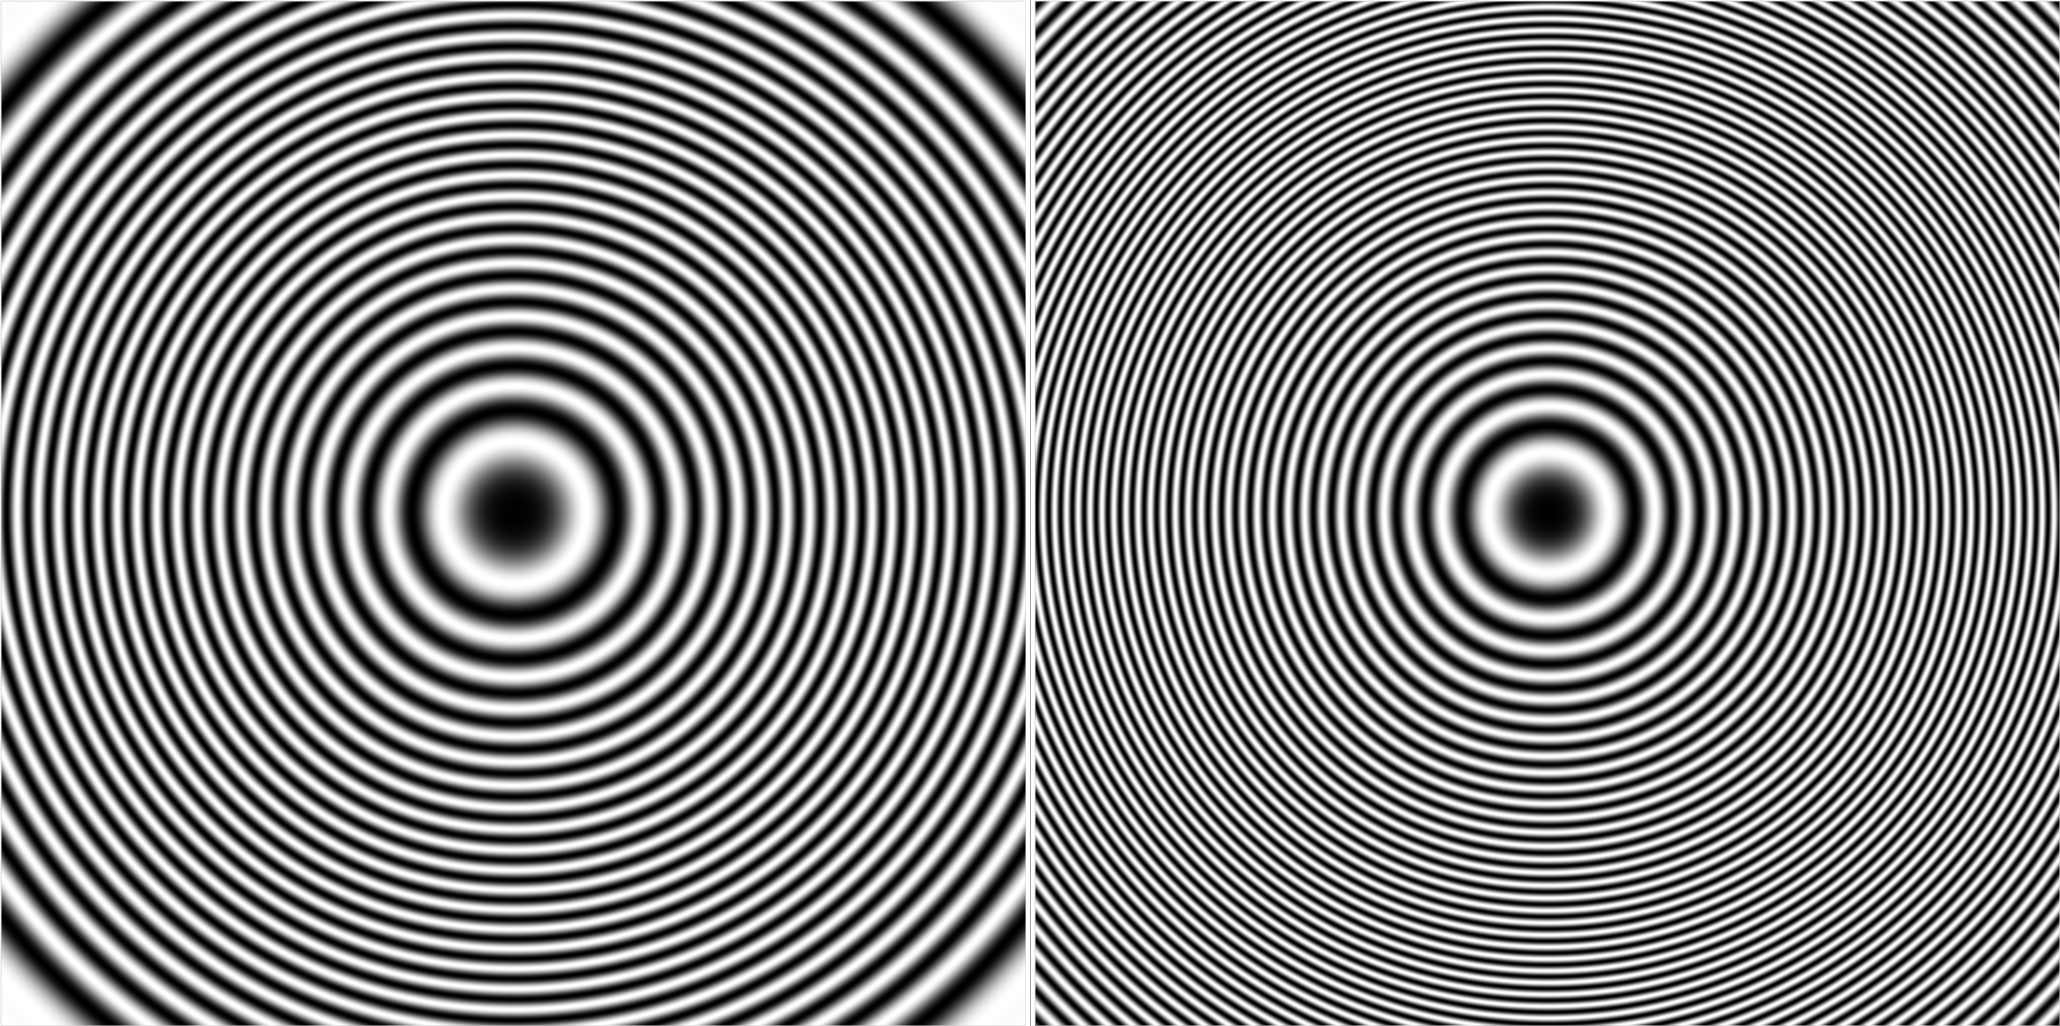
\includegraphics[width=\textwidth]{introduction/ctf_defocus_2d.png}
        \caption{2D power spectrum (|CTF|).}
        \label{fig:ctf_defocus_2d}
    \end{subfigure}%

    \begin{subfigure}{\textwidth}
        \centering
        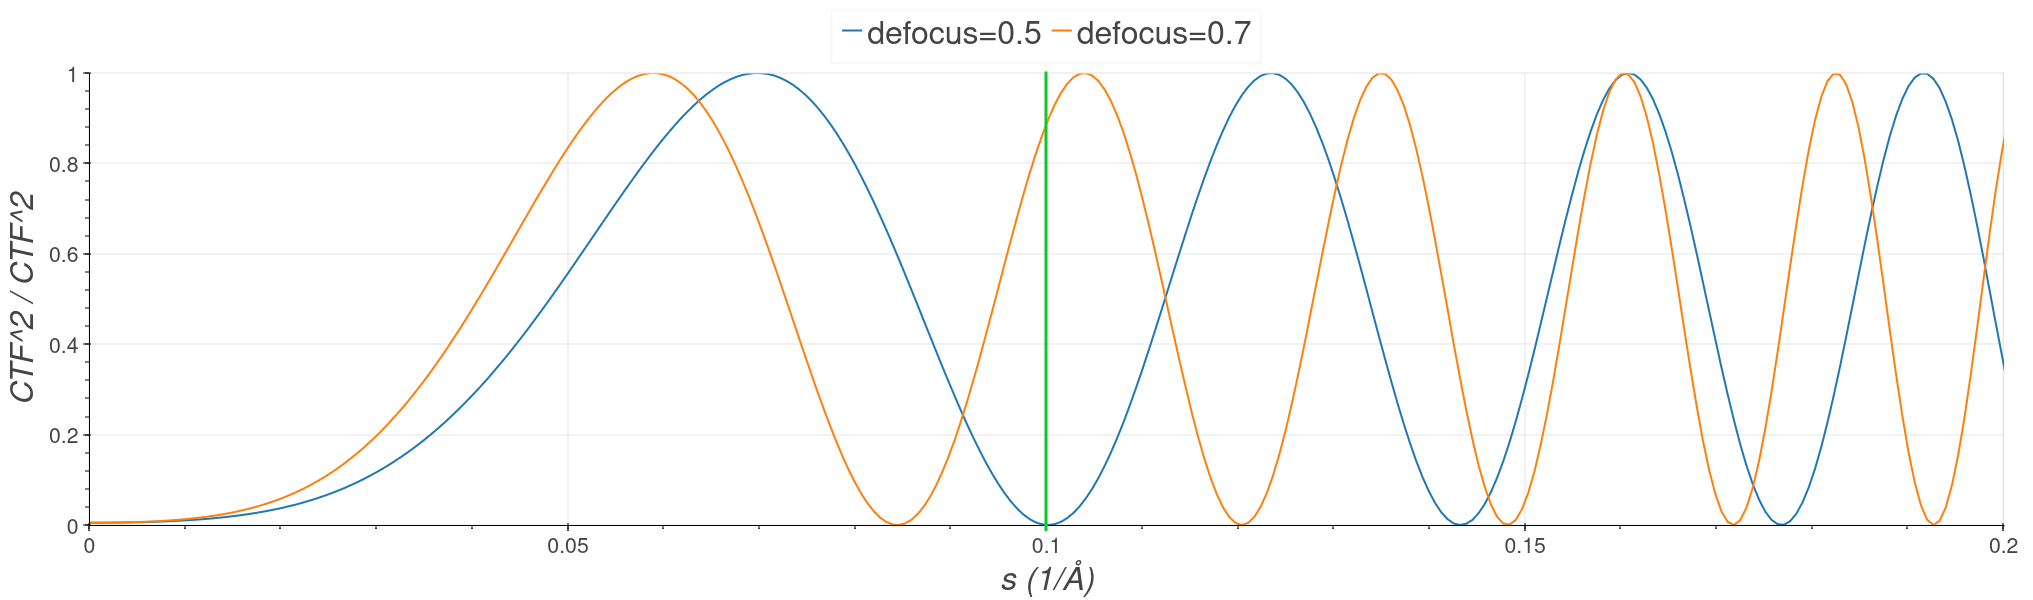
\includegraphics[width=\textwidth]{introduction/ctf_defocus_1d.png}
        \caption{1D rotational average.}
        \label{fig:ctf_defocus_1d}
    \end{subfigure}%

    \caption[CTF: effect of defocus]{Simulated CTF of two images at different defoci. Highlighted in green is the spatial frequency of \qty{0.1}{\angstrom^{-1}}, where there the blue line (CTF at defocus \qty{0.5}{\micro\meter}) is close to zero, whereas the orange line (CTF at defocus \qty{0.7}{\micro\meter}) is close to 1. Image generated with: \url{https://ctfsimulation.streamlit.app/}~\cite{jiangWebbasedSimulationContrast2001}.}
    \label{fig:ctf_defocus}
\end{figure}

To ensure all spatial frequencies are sampled, a data collection must therefore include many images collected at a range of different defoci.
Additionally, some defocus is always required for low resolution information to be visible; without it, particle identification and picking will be impaired.
Alternatively, a phase plate can be used to shift the phase of the electrons by 90 degrees and acquire images on focus (\autoref{fig:ctf_phase_shift}) CITE.

\begin{figure}[ht]
    \centering
    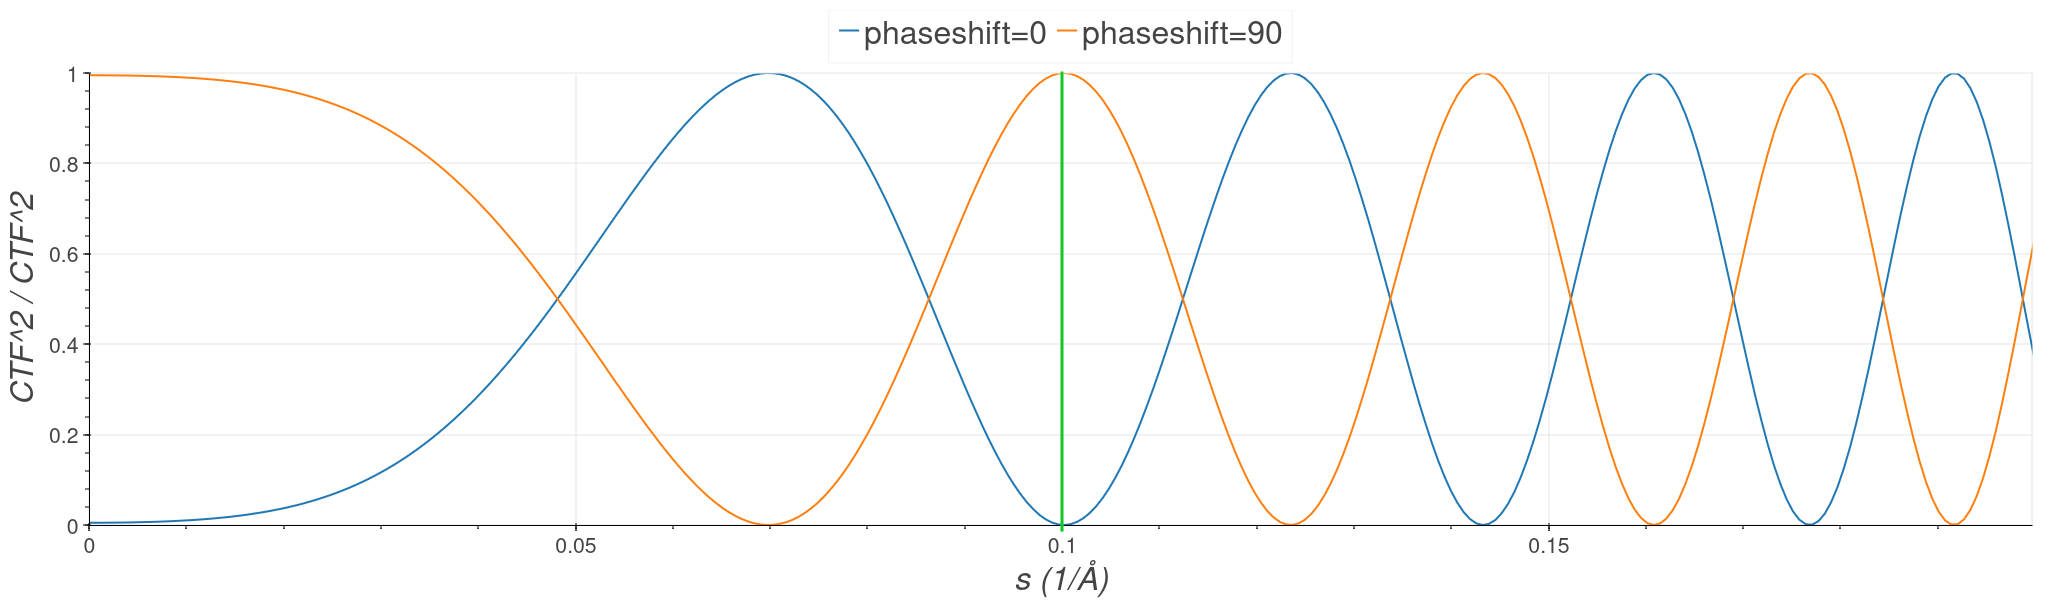
\includegraphics[width=\textwidth]{introduction/ctf_phase_shift.png}
    \caption[CTF: effect of phase shift]{Simulated CTF of two images at different phase shifts. Note how the phase-shifted CTF (orange) has a peak at spatial fequency \num{0}, boosting low-resolution features. Image generated with: \url{https://ctfsimulation.streamlit.app/}~\cite{jiangWebbasedSimulationContrast2001}.}
    \label{fig:ctf_phase_shift}
\end{figure}

Given the above examples, it may appear that it is possible to fully correct for CTF and get perfect signal.
However, due to noise and to the envelope function dampening high resolution oscillation, it's never possible to perfectly estimate the CTF parameters (\autoref{fig:ctf_envelope}).
Therefore, when correcting for CTF during processing, the wrong spatial frequencies will be boosted and dampened.
This mostly affects high-resolution information, where the CTF oscillation are faster and a small parameter error has greater impact.

\begin{figure}[ht]
    \centering
    \begin{subfigure}[B]{.42\textwidth}
        \centering
        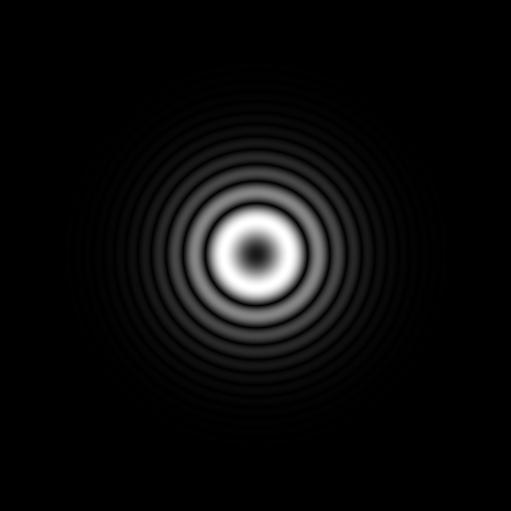
\includegraphics[width=\textwidth]{introduction/ctf_envelope_2d.png}
        \caption{2D power spectrum.}
        \label{fig:ctf_envelope_2d}
    \end{subfigure}%
    \hfill
    \begin{subfigure}[B]{.55\textwidth}
        \centering
        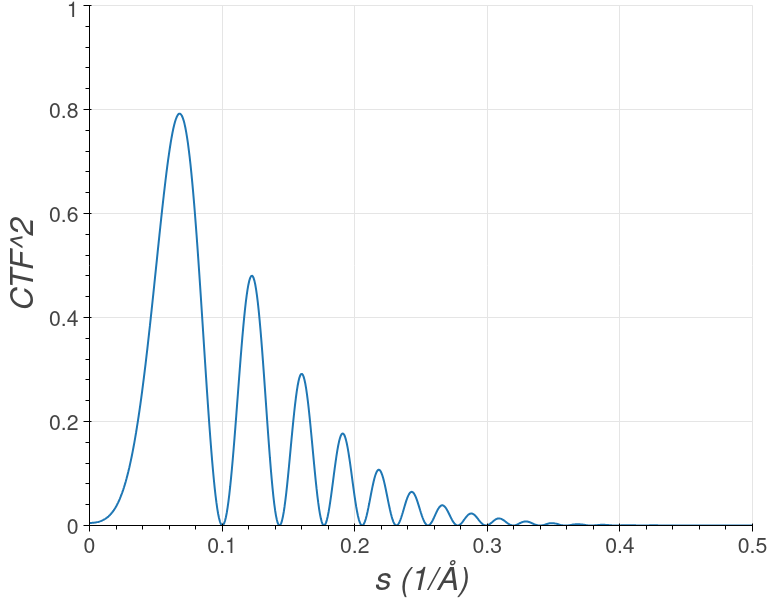
\includegraphics[width=\textwidth]{introduction/ctf_envelope_1d.png}
        \caption{1D rotational average.}
        \label{fig:ctf_envelope_1d}
    \end{subfigure}%
    \caption[CTF: effect of the envelope function]{Simulated CTF of an image, including some envelope function effects (such as beam convergence and energy spread). As a result, higher resolution frequencies are dampened, reducing the signal available for CTF estimation and high resolution reconstruction. Image generated with: \url{https://ctfsimulation.streamlit.app/}~\cite{jiangWebbasedSimulationContrast2001}.}
    \label{fig:ctf_envelope}
\end{figure}

TODO: delocalization of signal

(TODO: would be cool to link here somehow to my CTF simulator in napari... Though probably not worth discussing CTF so in depth that we explain fourier transforms and how they combine to form an image?)

\subsection{Preprocessing}

Before particle picking, classification and 3D reconstruction can be performed, the collected data must undergo a few preprocessing steps.

First, each movie generated during data collection must be aligned and averaged.
In state of the art applications, this alignment is typically done not only on a full frame level, but also in a localized fashion, by aligning image patches or by describing the system with a smooth deformation field~\cite{zhengMotionCor2AnisotropicCorrection2017} (CITE cryosparc, others?).

In state of the art software, similarly to how motion correction is treated, defocus (and thus CTF) is estimated at a local level, accounting for variability in the positioning of the sample with respect to the detector.
The parameters thus obtained are later used to correct for the CTF during classification and reconstruction.
Modern workflows also offer the ability to later refine the deformation parameters as part of the refinement process (see \nameref{refinement}).

The dataset often contains bad images for various reasons: too high motion, issues with autofocus, too thick or cracked ice, etc.
During preprocessing, these micrographs are usually discarded, either manually or by using batch automated tools which estimate the data quality.

Once the data is clean, motion corrected and CTF-estimated, the particles of interest can be picked for further processing.

\subsection{Particle picking}

In order reconstruct the 3D map of particles of interest, one first needs to locate them on the micrograph.
This is called particle picking, and can be performed with varying levels of automation, and using several different techniques.
The most commonly used are variations of manual picking, template matching, and machine learning (ML) tools.

Manual picking is more intuitive and can be very precise, but is also tedious and time-consuming.
Data may also be too noisy for humans to distinguish particles from one another and from the background, leading to missed particles or wrong picks.
To aid with manual picking, preprocessed micrographs are often filtered and denoised to improve the contrast (see \nameref{filtering_and_denoising}).

To improve the picking speed and precision, template matching is often used to automate searching for a recognizable object.
This picking method requires a template: a small 2D image of a projection...


either after a first round of manual picking or using a template generated from an existing known map of the object of interest or a similar structure.

\subsubsection{Filtering and denoising}\label{filtering_and_denoising}

TODO: also explain effects of high res and low res info on perceived contrast/readability.

\begin{figure}[ht]
    \centering
    \includegraphics[width=.5\textwidth]{example-image.png}
    \caption{TODO: Filtering/denoising side by side}
    \label{fig:filtering}
\end{figure}


\subsection{Refinement}\label{refinement}
...

\FloatBarrier

\begin{outline}
\1 Background on Cryo-EM in structural biology
    \2 Base concepts (do not spend too much time on this)
        \3 \tick sample prep
        \3 \tick exposure damage
        \3 \tick role of detectors and resolution revolution \cite{faruqiCCDDetectorsHighresolution2000}
        \3 \tick data collection
        \3 \tick image formation
        \3 \tick CTF
        \3 \tick defocus (and ranges of defocus) and info spread
        \3 \tick dataset cleaning
        \3 particle picking
        \3 2D classification and selection
        \3 typical processing steps, theory behind reconstruction and classification (more time here as it's more relevant for cryoet and my work)
        \3 single particle analisys
        \3 model building
    \2 typical use cases (some example of single particle data, maybe using ftsz images) and advantages
        \3 no crystal, simpler sample prep
        \3 heterogeneity to a certain extent
        \3 more native state
        \3 bigger targets? complexes
    \2 limitations (leading up to cryo-et) and comparison with other techniques (xray, nmr)
        \3 sample prep/thickness/denaturation
        \3 context missing
        \3 ability to capture dynamics/heterogeneity (more/less than other techniques)
        \3 Signal/Noise
\1 cryo-et, concepts and advantages
    \2 base concepts and differences from SPA from thechnical standpoint
        \2 cryoem, but different data acquisition and thus data processing
        \3 exposure damage and dose issues
        \3 sample prep (thinnes especially important because SNR)
        \3 tilt-series alignment (fiducials), deformation, other aberrations, how they are tackled
        \3 3D CTF
        \3 missing wedge, issues it introduces
        \3 feature deletion (e.g: fiducials)
        \3 segmentation/morphology
        \3 STA (picking, averaging, classification, ...) for non-unique objects (template matching, geometric and template free, machin learning)
    \2 some references/reviews (cool stuff you can do)
        \3 \cite{turkPromiseChallengesCryoelectron2020,lucicCryoelectronTomographyChallenge2013}
    \2 what it provides compared to SPA
        \3 more native state and context preservation
        \3 single-particle insights
        \3 meso-scale and superstructural information
    \2 limitations (both in terms of technique, and in terms of current state of development)
        \3 (some mentioned before, maybe need to connect these two parts a bit better)
        \3 need for custom workflow cause the goal and problems are usually unique
        \3 issues caused by the missing wedge (alignement, reconstruction, interpretability)
        \3 SNR, denoising
        \3 visualisation/interaction
        \3 object identification (crowding
    \2 related techinques to overcome some limitations
        \3 FIB, what it enables and how it works
        \2 CLEM
\end{outline}
